\chapter{Auswertung und Diskussion}
\label{sec:aus}

Im Folgenden werden die experimentellen Messwerte aufgeführt und diskutiert. 
Zu Beginn wird in \autoref{sec:SN} das Rauschen des Aufbaus festgestellt und die Abhängigkeit 
von der Zeitkonstante des Lock-In-Verstärkers geprüft. 
Als weitere Vorbereitung wird die Größe des Strahls mithilfe des 
Rasierklingen-Verfahrens bestimmt und anschließend mit den 
daraus bestimmten Werten die Leistung pro Flächeneinheit berechnet.
Anschließend werden in \autoref{sec:AZnTe} Referenzwerte für die THz-Erzeugung bestmmimmt, 
indem die Transienten sowie deren Fouriertransformierten 
ausgewertet werden. 
Dazu wird das Verhalten der Amplituden 
bei verschiedenen Laserleistungen analysiert. 
Diese Schritte werden anschließend für die zwei organischen Kristalle OH1 und BNA in \autoref{sec:AOH1} und \autoref{sec:ABNA} wiederholt 
und mit den bekannten Werten aus \autoref{sec:AZnTe} verglichen.


\section{Bestimmung des Rauschuntergrunds}
\label{sec:SN}
Das Rauschen wird in verschiedenen Situationen gemessen, 
wobei zwischen Netzspannungs- und 
Batterieversorgung unterschieden wird.
Diese Unterscheidung wird getroffen, um Störquellen wie Erdschleifen und Netzbrummen 
von dem intrinsischen Elektronikrauschen der Photodioden zu trennen. 
Bei der Netzspannung wird dazu das Rauschen bei 
eingeschaltetem wie auch bei ausgeschaltetem Laser gemessen. \\



% Um das Rauschen zu prüfen wird ausschließdlich der Probe-Strahl durch den Aufbau gelassen und 
% der Pump-Strahl geblockt. 
% Dadurch entsteht im Detektionskristall keine änderung der Polarisations und die beiden 
% anteile die vom Wollaston-Prisma erzeugt werden sind identisch. 
% Somit sollte das gemessene Signal Theoretisch 0 Ergeben. 
% Dazu wurde dies einmal ganz ohne beleuchtung durchh den Laser durchgefühhrt um den unterschied 
% zwischen Rauschen nur durch den aufbau zu sehen und das Rauschen welches durchh den laser selber 
% hinzugefüt wird weil dieser auch nicht pefekt funktioniert.


In \autoref{fig:tc1} sind die Werte für die Messungen mit Netzspannung, mit jeweils eingeschaltetem und ausgeschaltetem Laser zu sehen. 
In den Messungen mit eingeschaltetem Laser wird jedoch nur der 
Detektionsstrahl 
freigegeben, während der Pumpstrahl blockiert ist, 
sodass auch hier ausschließlich das Rauschen gemessen wird.
Anschließend wird die Zeitkonstante $\tau$ von 
$\SIrange{30}{3000}{\milli\second}$ am Lock-In-Verstärker variiert. 
Bei jeder Zeitkonstante wird $\SI{20}{s}$ lang gemessen und 
anschließend der Mittelwert bestimmt. 

\begin{figure}
    \centering
    \begin{subfigure}[b]{0.48\textwidth}
        \centering
        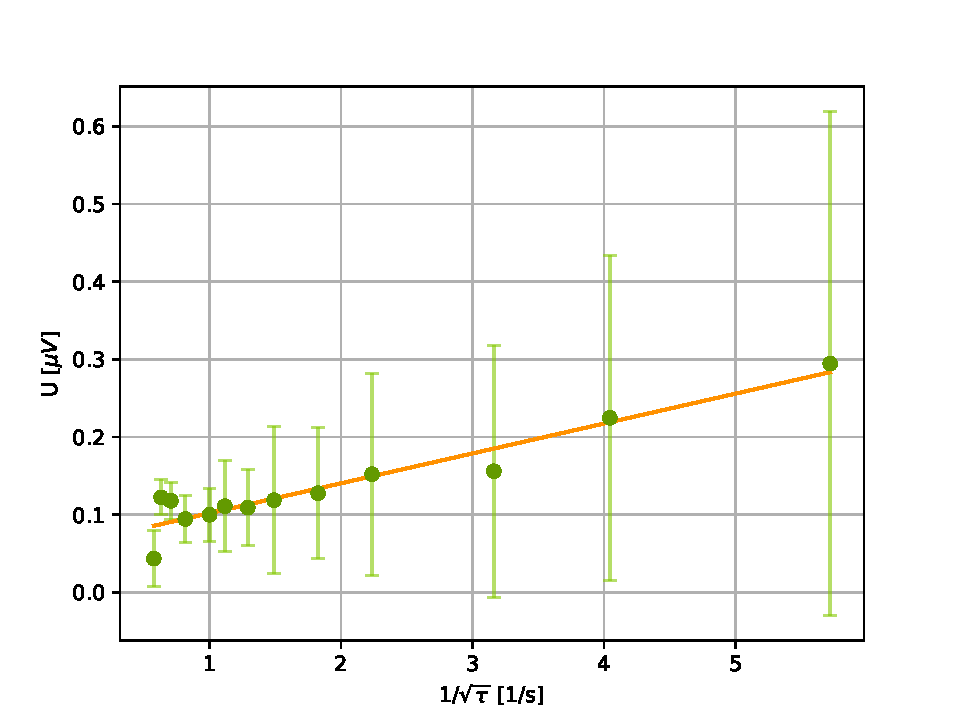
\includegraphics[width=\textwidth]{content/plots/pdf/time_constant/time_constant_oi.pdf}
        \caption{Ohne Beleuchtung.}
        \label{fig:tco}
    \end{subfigure}
    \hfill
    \begin{subfigure}[b]{0.48\textwidth}
        \centering
        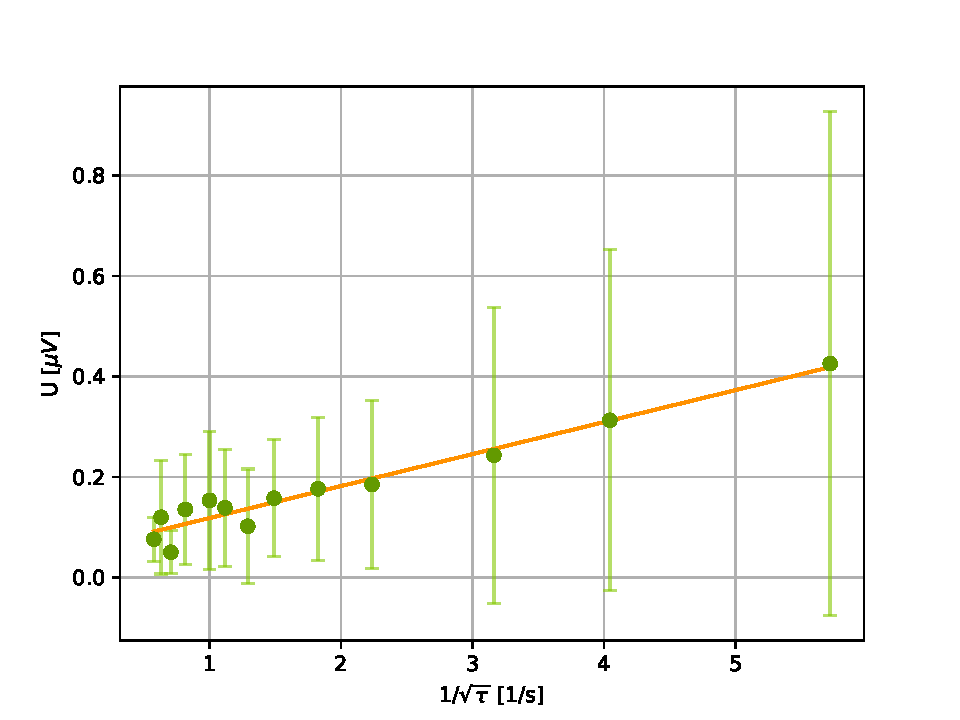
\includegraphics[width=\textwidth]{content/plots/pdf/time_constant/time_constant_wi.pdf}
        \caption{Mit Beleuchtung.}
        \label{fig:tcw}
    \end{subfigure}
    \caption{Durchschnitt der Messwerte der Rauschspannung über $\SI{20}{\second}$ gegen $\frac{1}{\sqrt{\tau}}$ aufgetragen. An beiden Reihen 
    ist eine Ausgleichsgerade der Form $\frac{A}{\sqrt{\tau}}$ angelegt.}
    \label{fig:tc1}
\end{figure}
 
In \autoref{fig:tco} sind
die Daten ohne Beleuchtung durch den Detektionsstrahl zu sehen und in 
\autoref{fig:tcw} mit Beleuchtung. 
Dazu wurde bei beiden ein Fit gemäß \autoref{eqn:tc} durchgeführt, wobei $A$ die Rauschamplitude 
der Messung ist. 
Für die Fit-Werte ergeben sich 
\begin{align}
    \label{tab:tc1}
    A_\text{Ohne} =&\SI{59.2+-5.2}{\nano\volt} \\
    A_\text{Mit} =&\SI{81.5+-4.9}{\nano\volt} \, .
\end{align}
Es zeigt sich, dass die Rauschamplitude ohne Beleuchtung um $27\%$ kleiner ist als 
mit Beleuchtung. 
Dieser Faktor lässt sich damit erklären, dass bei Lichteinstrahlung 
an den Photodioden das Schrotrauschen hinzukommt. 
Das Schrotrauschen ist eine Folge der Quantisierung des Lichts. 
Denn die Photonen treffen zu zufälligen, statistisch unabhängigen Zeitpunkten auf die Photodioden, 
sodass die Zahl der pro Zeitintervall erzeugten Ladungsträger Poisson-verteilt ist, 
wodurch eine weitere Unsicherheit in den Messprozess hinzukommt.
Aus dem Rauschen bei eingeschaltetem Laser lässt sich zusätzlich das
Signal-Rausch-Verhältnis bezogen auf ein Referenzsignal von $\SI{45}{\milli\volt}$
für die verschiedenen Zeitkonstanten bestimmen, die Werte sind in \autoref{tab:snr_wi}
aufgelistet.
Das Referenzsignal ist die Spannung einer einzelnen Photodiode bei eingeschaltetem Detektionsstrahl ohhne THz-Feld, 
also wenn auf beiden Dioden die selbe Spannung liegt. 


\begin{table}
    \centering
    \caption{Aus dem Rauschen $U$ bei eingeschaltetem Laser (Netzspannung) berechnetes
    Signal-Rausch-Verhältnis, bezogen auf ein Referenzsignal von $\SI{45}{\milli\volt}$,
    für verschiedene Zeitkonstanten $\tau$ des Lock-In-Verstärkers.}
    \label{tab:snr_wi}
    \begin{tabular}{S[table-format=4.1] S[table-format=3.1] S[table-format=6.0]}
        \toprule
        {$\tau \mathrel{/} \si{\milli\second}$} & {$U \mathrel{/} \si{\nano\volt}$} & {SNR}  \\
        \midrule
        30.6   & 425.6 & 105738 \\
        61.2   & 312.8 & 143863 \\
        100.0  & 243.1 & 185122 \\
        200.0  & 184.9 & 243329 \\
        300.0  & 176.4 & 255169 \\
        449.8  & 157.8 & 285094 \\
        599.4  & 102.1 & 440898 \\
        800.4  & 138.6 & 324750 \\
        998.2  & 153.5 & 293120 \\
        1500.0 & 135.3 & 332607 \\
        2000.0 & 50.2  & 896338 \\
        2500.0 & 119.9 & 375395 \\
        3000.0 & 76.0  & 592457 \\
        \bottomrule
    \end{tabular}
\end{table}



Die Messung der Rauschspannung wird wiederholt, wobei die
Stromversorgung der Photodioden nicht von 
Labornetzgeräten, welche mit Netzstrom betrieben werden, 
sondern mit Batterien versorgt werden. 
Um zusätzlich den Einfluss der Messdauer zu prüfen, wird einmal über 
$\SI{20}{\second}$ gemittelt und einmal über $\SI{60}{\second}$. 
Die sich daraus ergebenden Werte sind in \autoref{fig:tc2} zu sehen. 
Dabei ist \autoref{fig:tc20} die Darstellung der Mittelwerte aus der $\SI{20}{\second}$-Serie mit einer Messdauer von 
$\SI{20}{\second}$, 
\autoref{fig:tc60} der Graph für $\SI{60}{\second}$. 
An beide Mittelwertensembles wird eine Ausgleichsgerade, \autoref{eqn:tc} gelegt. 
% Hierbei ist zu berücksichtigt, dass der Messwert mit der 
% niedrigsten Zeitkonstante ($\tau= \SI{30}{\milli\second}$) 
% aufgrund des sehr großen Fehlers und einem abweichen. 



\begin{figure}
    \centering
    \begin{subfigure}[b]{0.48\textwidth}
        \centering
        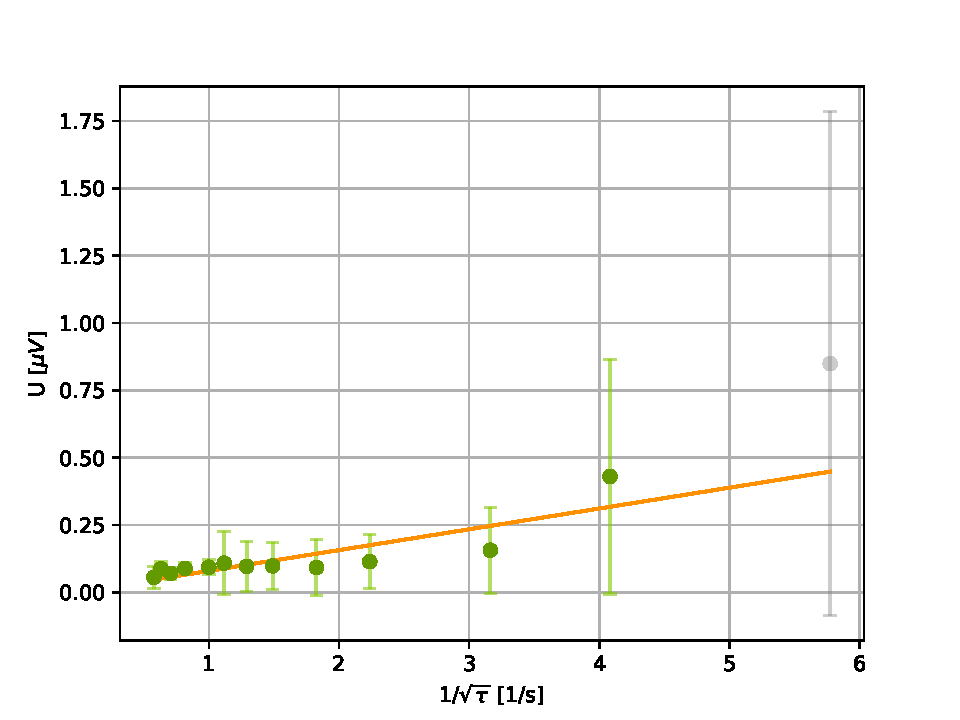
\includegraphics[width=\textwidth]{content/plots/pdf/time_constant/time_constant_b20.pdf}
        \caption{Messung mit einem Messintervall von $\SI{20}{\second}$.}
        \label{fig:tc20}
    \end{subfigure}
    \hfill
    \begin{subfigure}[b]{0.48\textwidth}
        \centering
        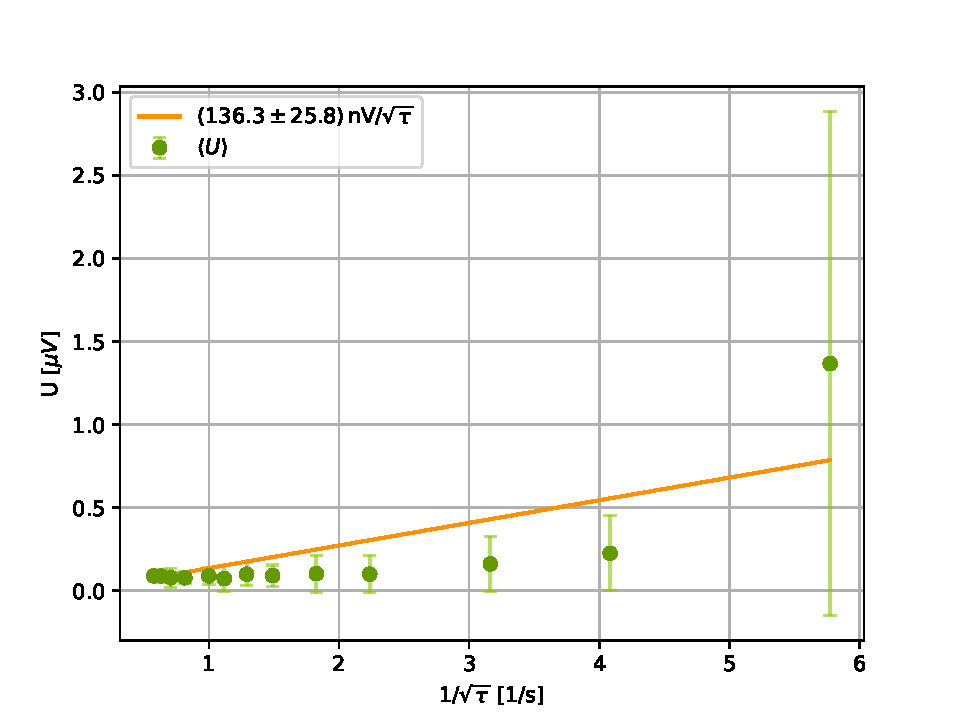
\includegraphics[width=\textwidth]{content/plots/pdf/time_constant/time_constant_b60.pdf}
        \caption{Messung mit einem Messintervall von $\SI{60}{\second}$.}
        \label{fig:tc60}
    \end{subfigure}
    \caption{Messwerte der Rauschspannung bei Stromversorgung per Batterie bei keiner Beleuchtung durch den Laser,
        mit je einer Ausgleichsgerade, der Form $\frac{A}{\sqrt{\tau}}$.}
    \label{fig:tc2}
\end{figure}
 
Die aus der Ausgleichsgerade resultierenden Werte sind 

\begin{align}
    \label{tab:tc2}
    A_\text{20\,s} =&\SI{108.5+-11.4}{\nano\volt}  \\
    A_\text{60\,s} =&\SI{136.3+-25.8}{\nano\volt} \, .
\end{align}

Durch die Werte lässt sich zeigen, dass die 
Rauschamplitude bei den Batterien und einem $\SI{20}{\second}$‑Messintervall um $83\%$ größer ist als die $\SI{20}{\second}$ mit 
Netzspannung und ohne beleuchtung. 
Die Rauschamplitude bei dem langen, $\SI{60}{\second}$, Messintervall ist $26\%$ größer als bei dem kurzen Messintervall und Baterie versorgung.
Hinzu kommt, dass die Rauschamplitude $A_\text{60\,s}$ bei 
Batterieversorgung $130\%$ größer ist als bei Netzversorgung und $\SI{20}{\second}$-Messintervall. 
Zusammengefasst sind die gesamten Messdaten in \autoref{fig:tcc}. 
Diese zeigen, dass das Rauschen bei steigender Zeitkonstante $\tau$ abnimmt 
und ab 
$\tau=\SI{0.5}{\second}$ ein Plateau erreicht, bei welchem sich das Rauschen nur minimal ändert. 
Bereits zu Beginn ist das Rauschen bei 
eingeschaltetem Laser und niedrigen 
Zeitkonstante höher als bei ausgeschaltetem Laser. 
Erklären lässt sich dies durch das Schrotrauschen. 
\begin{figure}
    \centering
    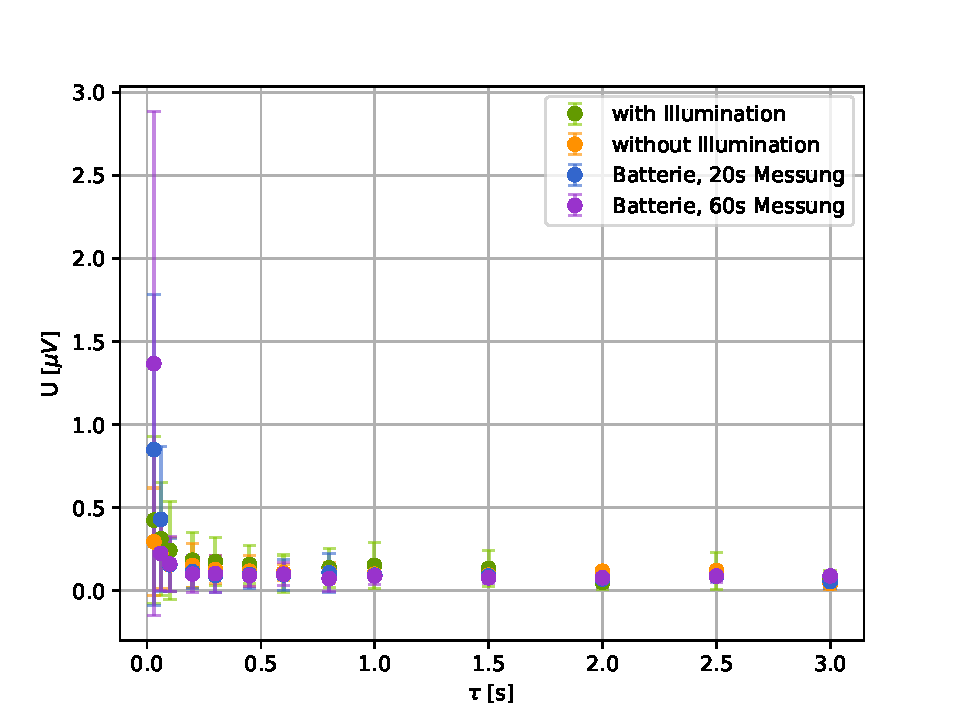
\includegraphics[width=0.8\textwidth]{content/plots/pdf/time_constant/time_constant_combined_vs_tau.pdf}
    \caption{Vergleich der Rauschspannung mit und ohne eingeschaltetem Laser.
    Dazu die Werte mit der Batterie als Stromversorgung bei verschiedenen Mittelungszeiten.
    In grün und orange siind die Messreihen mit den Labornetzgeräten als Stromversorgung aufgetragen, 
    in blau und violet die mit Batterie als Stromquelle.}
    \label{fig:tcc}
\end{figure}


Dieser statistische Prozess lässt sich durch eine längere 
Zeitkonstante herausmitteln, wodurch das Rauschen bei höheren 
Zeitkonstanten abnimmt.




Ab eine Zeitkonstante von $\tau=\SI{0.5}{\second}$ ist keine große änderung des Rauschens zu sehen. 
Deswegen wird in dieser Bachelorarbeit mit einer Zeitkonstante von 
$\tau=\SI{0.1}{\second}$ gearbeitet, 
wobei aber fünf Messungen am selben Ort genommen 
werden. Effektiv ist dies eine Zeitkonstante von 
$\SI{0.5}{\second}$. 
Dieses Vorgehen wurde gewählt um den Messvorgang zu beschleunigen, 
da das Messprogramm vor jeder Einzelmessung einige Zeitkonstanten abwartet, 
bevor es misst. 
Durch die kürzere Einzelzeitkonstante wird diese Wartezeit verringert, 
während die 
Qualität der Messdaten durch die anschließende Mittelung über 5 
Messungen erhalten bleibt. 


% Erklären lässt sich das dadurch, dass der Laser statistische Prozesse 
% wie das Schrotrauschhen auslößt und somit eine weitere untsicherheit in die messung hereinbringt.
% Der Offsetwert $b$ ist nahzu identisch und liegt innerhalb des Fehlers. 
% Somit kann angenommen werden, dass das Grundrauschen nur von der Eleketronik abhängt unnd nicht 
% vom Laser Strahl abhängt.

% Dazu ist in \autoref{fig:tcc} ein vergleich von den beiden Messreihen zu sehen. 
% Dort ist zu sehen, dass zu begin der Unterschied noch gut zu sehen ist, aber mit höherer 
% Zeitkonstante immer weniger wird und ab ungeähr einer Zeitkonstante von $0,8\,\unit{s}$ nicht 
% mehr überhuapt sicher festgestellt werden kann. 
% Somit ergibt sich für die Restlichen Messungen, dass eine Zeitkonstante von mindestens 
% $0,8\,\unit{s}$ gewählt werden sollte.
% zeigen, dass für die folgende Messung eine Zeitkonstante $\tau \ge 0,8\,\unit{s}$ sinvoll 
% ist, damit das Rauschhen durch zum beispiel schrotrauschen hehrausgemittelt wird und eine 
% möglichst Rauschfreie Messung durchgeführt werden kann.

%--------------------------------------------Abschnitt Spot größe
\section{Bestimmung der Strahlgröße}
\label{sec:spot}
Da die organischen Kristalle äußerst klein sind und der Laserstrahl hingegen deutlich größer ist, 
wird im Folgenden die Größe des Laserstrahls bestimmt, mit welcher anschließend die Leistungsdichte bestimmt werden kann. 
Diese Werte gelten in den folgenden Kapiteln als Referenz für die einwirkende Leistung auf die Kristalle. \\
Um die Strahlgröße zu bestimmen, wird das Rasierklingen-Verfahren verwendet \cite{mohamed2019measurements}. 
Bei diesem wird senkrecht zum Strahl eine Rasierklinge an einer verstellbaren Plattform angebracht und in den Strahl bewegt. 
Dieser Aufbau wird an der Stelle platziert, an der auch die Generationskristalle platziert werden. 
Hinter dieser Stelle wird die Leistung gemessen. 
Um die Strahlgröße zu bestimmen, wird die Rasierklinge in $\SI{0.05}{\milli\meter}$ Schritten verschoben, sodass 
mehr Strahlanteile von der Klinge blockiert werden und die gemessene Leistung entsprechend sinkt. 
Für jede Verstellung wird die Differenz der Leistung zweier aufeinanderfolgender Messwerte bestimmt. 
Diese Differenz entspricht näherungsweise der Leistung, die auf die in diesem Schritt zusätzlich abgeschnittene Fläche entfällt.
Diese Differenz wurde jeweils in $x$- und $y$-Richtung bestimmt. 
Die Messdaten dazu sind in \autoref{fig:spot_c} zu sehen. 
 
\begin{figure}
    \centering
    \begin{subfigure}[b]{0.48\textwidth}
        \centering
        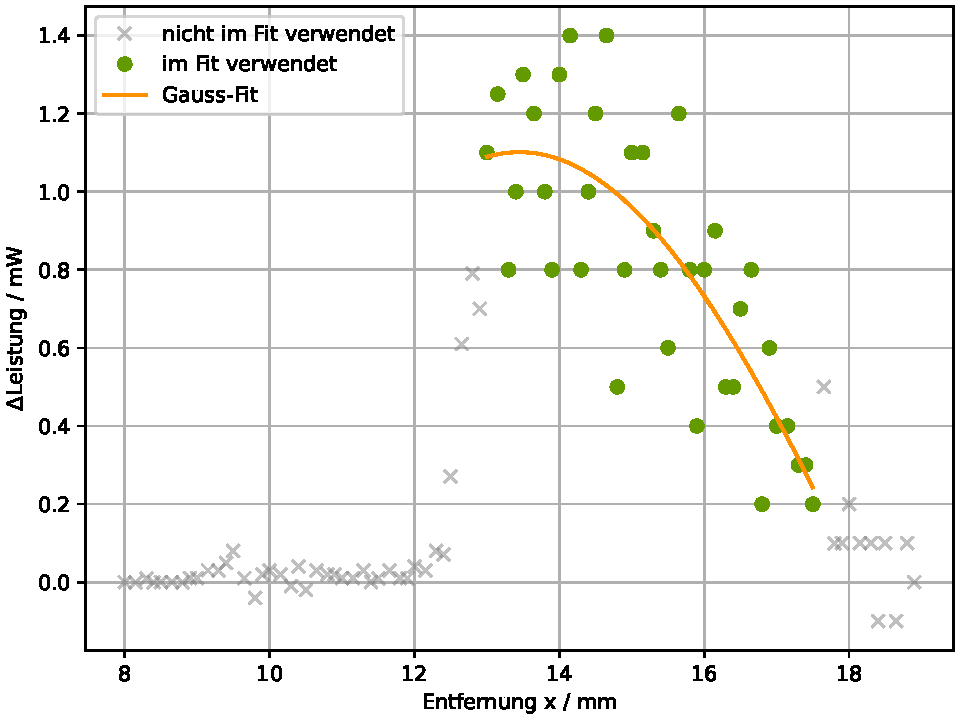
\includegraphics[width=0.8\textwidth]{content/plots/pdf/spot_size_x.pdf}
        \caption{$x$-Richtung.
        }
        \label{fig:spot_x}
    \end{subfigure}
    \hfill
    \begin{subfigure}[b]{0.48\textwidth}
        \centering
        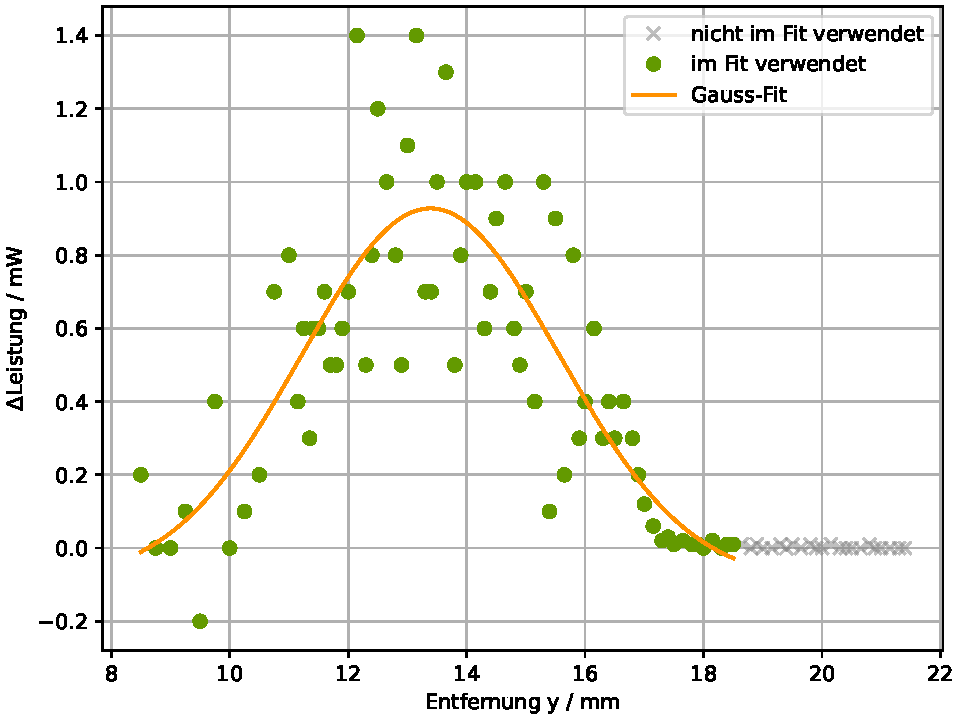
\includegraphics[width=0.8\textwidth]{content/plots/pdf/spot_size_y.pdf}
        \caption{$y$-Richtung.}
        \label{fig:spot_y}
    \end{subfigure}
    \caption{Ableitung der gemessenen Leistung bei Verschiebung der Rasierklinge entlang verschiedener Achsen.}
    \label{fig:spot_c}
\end{figure}


In \autoref{fig:spot_x} bzw. \autoref{fig:spot_y} sind die Differenzen der Leistung für die $x$- und $y$-Richtung zu sehen,
an welche jeweils ein Gauss-Fit der Form
\begin{equation}
    f(x) = A\cdot \exp\left(-\frac{1}{2}\left(\frac{x-\mu}{\sigma}\right)^2\right) + b
\end{equation}
angelegt wird.
Mithilfe des Fits ergeben sich die Koeffizienten
\begin{align}
    A_x &= \SI{9.20+-0.33}{mW/mm} & \mu_x &= \SI{14.62+-0.05}{mm} \\
    \sigma_x &= \SI{1.57+-0.08}{mm} & b_x &= \SI{-0.14+-0.23}{mW/mm} \\
    A_y &= \SI{7.80+-0.22}{mW/mm} & \mu_y &= \SI{13.42+-0.05}{mm} \\
    \sigma_y &= \SI{2.07+-0.08}{mm} & b_y &= \SI{-0.23+-0.16}{mW/mm} \,.
\end{align}
Aus der Standardabweichung des gaußförmigen Intensitätsprofils ergibt sich der Strahlradius als $w=2\cdot\sigma $.
Dieser Radius ist der, bei welchem die Intensität des Strahls bei $\frac{1}{e^2}$ der maximalen Intensität des Strahls ist \cite{mohamed2019measurements}.
Es ergeben sich
\begin{align}
	w_x &= \SI{3.15+-0.15}{\milli\meter} \ \\
	w_y &= \SI{4.14+-0.16}{\milli\meter} \, .
\end{align}
Es zeigt sich, dass der Strahl in $y$-Richtung eine etwas größere Ausdehnung besitzt als in $x$‑Richtung. Der Strahl ist also leicht elliptisch.
Für den Flächeninhalt wird daher $A =\pi w_x w_y$ genutzt.
Daraus errechnet sich der Flächeninhalt mit $\SI{41.15+-2.65}{\milli\meter\squared}$.
Die Leistung des Strahls an dieser Stelle beträgt $\SI{34.5}{\milli\watt}$.
Daraus lässt sich mit $I= \frac{P}{A}$ die mittlere Intensität
$\SI{0.838+-0.054}{\milli\watt\per\milli\meter\squared}$ bestimmen \cite{mohamed2019measurements}.
Dazu sei erwähnt, dass dies die durchschnittliche Intensität ist.
Der Laser ist aber ein Pulslaser und somit ist die Leistung eines einzelnen Pulses 
durch $\frac{\SI{34.5}{\milli\watt}}{\SI{3000}{\hertz}\cdot \SI{30}{fs}}\approx \SI{383}{MW}$ gegeben.
Die Leistung pro Puls ergibt sich aus der gemessenen Leistung des Lasers an der Generationskristallposition, 
geteilt durch die Pulsfrequenz mal der Puls Dauer.
Als Vergleichswert dient die kontinuierlich von dem Leistungsmesser gemessene Leistung aber trotzdem, da alle Messwerte mit demselben Laser aufgenommen wurden und somit über diesen 
Wert vergleichbar sind.
Dieser Wert pro Flächeninhalt wird verwendet, da die OH1- und BNA-Proben nicht den gesamten Strahl ausfüllen und so die Messwerte 
nicht mit denen von ZnTe, welcher 
den gesamten Strahl ausfüllt, vergleichbar wären. 
Im Folgenden wird die Referenzmessung mit ZnTe beschrieben.

\section{THz-Generation mit ZnTe}
\label{sec:AZnTe}
Um einen Vergleich für die organischen Emitter zu haben, wird zu Beginn eine Messung der THz-Strahlung, welche von 
ZnTe erzeugt wird, durchgeführt. 
Im Gegensatz zu den anderen Kristallen konnte die gesamte Fläche des Pumpstrahls zur Erzeugung genutzt werden, da der 
ZnTe-Kristall groß genug ist, um den gesamten Strahl auszufüllen. 
Zu Beginn wird die Position der Verzögerungsstrecke, an der die größte Amplitude des THz-Pulses auftritt, bestimmt. 
Anschließend wird um diesen Wert ein Intervall von $\SI{-4}{ps}$ bis $\SI{11}{ps}$ gemessen. 
Dieser Transient für eine Pump-Leistung von $\SI{55}{mW}$ ist in \autoref{fig:ZnTeT} zu sehen. 
In diesem ist die Zeit-Null bei $\SI{0}{ps}$ eingetragen und anschließend sind die Nachschwingungen zu sehen. 
Diese entstehen, da das Wasser in der Luft Teile des Pulses absorbiert und wieder emittiert, was zur Folge hat, dass der Puls auseinanderläuft.
Somit trifft ein geringer Teil erst später auf den Detektionskristall und wird so auch erst später gemessen.



\begin{figure}
    \centering
    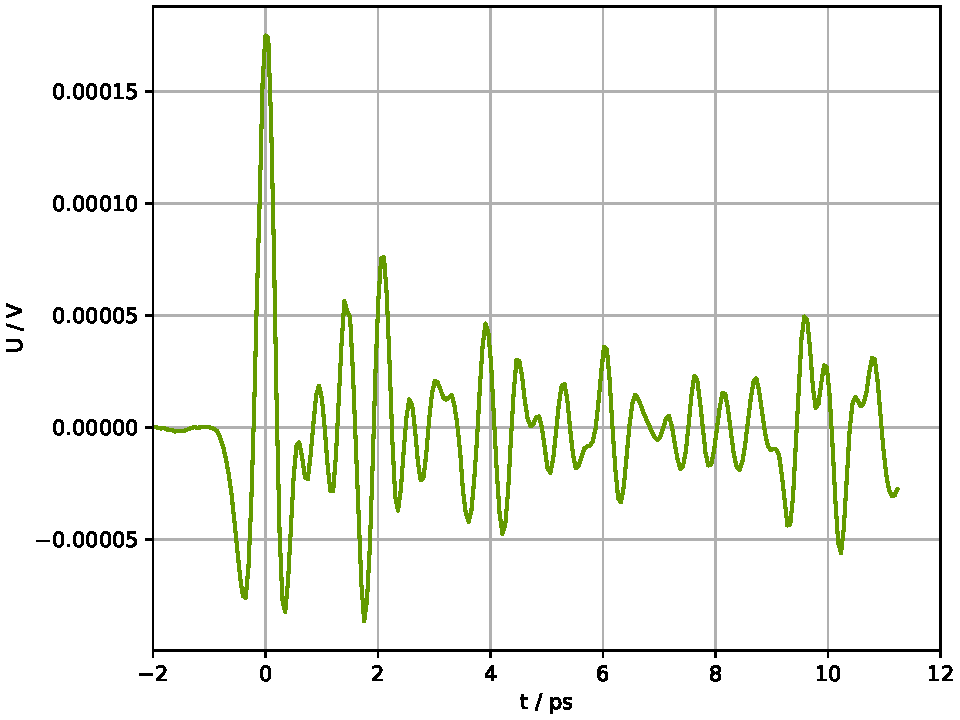
\includegraphics[width=0.8\textwidth]{content/plots/pdf/ZnTe/110mW.pdf}
    \caption{Transient des THz-Pulses, erzeugt von ZnTe, bei einer Pump-Leistung von $\SI{55}{\milli\watt}$.}
    \label{fig:ZnTeT}
\end{figure}

Dieser Transient wurde für verschiedene Pump-Leistungen gemessen und die Maximalwerte wurden bestimmt. 
In \autoref{fig:ampc} sind diese Werte aufgelistet und mit einem linearen Fit versehen, um die lineare Abhängigkeit von der 
Laserleistung zu prüfen. 
Auffällig dabei sind die Werte zwischen $\SI{30}{\milli\watt}$ und $\SI{48}{\milli\watt}$. Hier ist ein Anstieg zu den 
anderen Werten bei der Maximalwert zu sehen. Zwischen diesen und den anderen Messungen wurden verschiedene Spannungsquellen für die 
Photodioden geprüft, wobei diese sich nicht als ideal herausgestellt haben und zur Netzspannung zurückgewechselt wurde. 
Es scheint, als wäre im Zuge dessen die Einstellung an den Spannungsquellen verstellt worden, was die plötzlich höheren Werte der 
Messung erklären könnte.
Es ist anzumerken, dass die Leistung von $\SI{55}{mW}$ nicht die höchstmögliche Leistung des Lasers ist, aber ab dieser Leistung 
der Kristall anfängt lumineszent zu werden, was ein Zeichen für die Nähe der Zerstörschwelle ist. 
Um den Kristall nicht zu beschädigen, wurde deshalb die Leistung nicht weiter erhöht. 


% \begin{table}
%     \centering
%     \caption{Peak-to-Peak-Amplitude und daraus bestimmtes Signal-Zu-Rausch-Verhältnis der ZnTe-Transienten bei verschiedenen Pumpleistungen, bezogen auf die einheitliche Rauschreferenz $U_\text{Rausch}=\SI{0.158}{\micro\volt}$ bei $\tau=\SI{450}{ms}$.}
%     \label{tab:snZnTe}
%     \begin{tabular}{S[table-format=3.0] S[table-format=3.1] S[table-format=4.1]}
%         \toprule
%         {$P \mathrel{/} \si{\milli\watt}$} & {$U_\text{ptp} \mathrel{/} \si{\micro\volt}$} & {SNR} \\
%         \midrule
%         2   & 15.4  & 97.3   \\
%         3,3  & 18.7  & 118.5  \\
%         7,4  & 46.9  & 296.6  \\
%         8  & 77.5  & 490.7  \\
%         13  & 88.8  & 561.9  \\
%         18  & 116.2 & 735.3  \\
%         24  & 143.7 & 909.2  \\
%         30  & 261.3 & 1653.7 \\
%         34  & 306.2 & 1938.0 \\
%         40  & 353.8 & 2239.4 \\
%         48  & 386.7 & 2447.7 \\
%         55 & 261.4 & 1654.3 \\
%         \bottomrule
%     \end{tabular}
% \end{table}



Des Weiteren wird eine Fourier-Transformation mit den Transienten durchgeführt. Diese ist für eine Anregungsleistung von $\SI{55}{mW}$ in \autoref{fig:ZnTeF} zu sehen.
Die Fouriertransformierte zeigt, welche Frequenzen in dem Transienten des THz-Pulses vorhanden sind. 
Aus diesem lässt sich die Bandbreite von dem THz-Puls bestimmen. 
Diese beträgt $\SI{2.4}{\tera\hertz}$.
Wobei Frequenzen zwischen $\SI{0.2}{\tera\hertz}$ und $\SI{2.6}{\tera\hertz}$ erzeugt werden. 
Besonders hervorzuheben sind die zwei Absorptionslinien bei $\SI{1.2}{THz}$ und $\SI{1.7}{THz}$ \cite{HITRAN2020}. 
Diese Einbrüche entstehen durch die Absorption von THz im Wasser, welches in der Luft als Wasserdampf 
vorhanden ist.


\begin{figure}
    \centering
    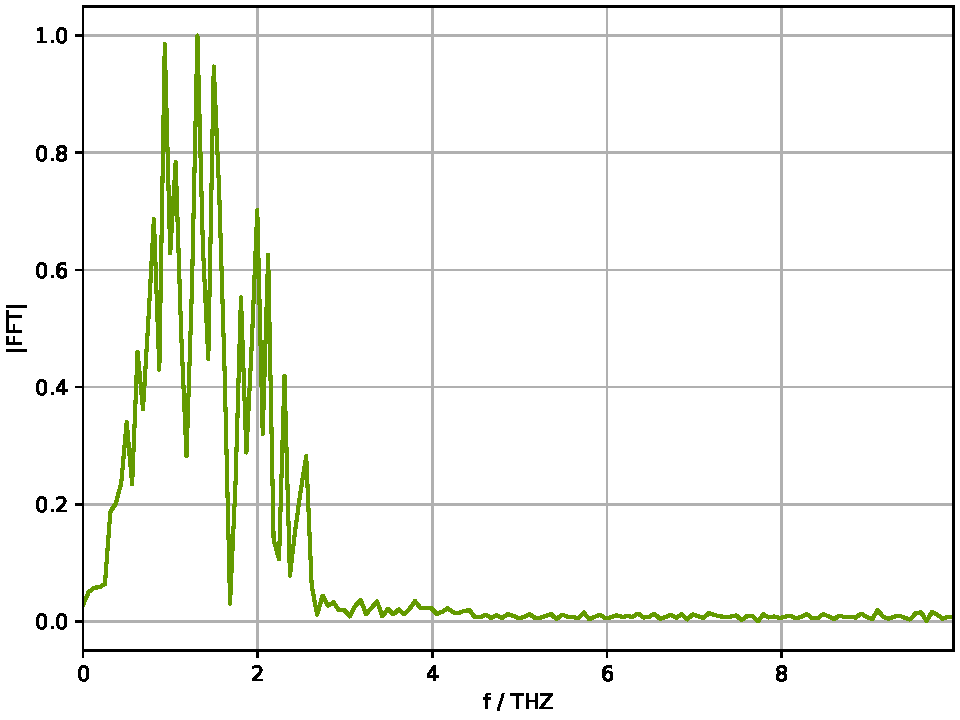
\includegraphics[width=0.8\textwidth]{content/plots/pdf/ZnTe/110mW_fft.pdf}
    \caption{Fouriertransformierte des THz-Pulses, erzeugt von ZnTe, bei einer Pump-Leistung von $\SI{55}{\milli\watt}$.
    Bei $\SI{1.2}{\tera\hertz}$ und $\SI{1.7}{\tera\hertz}$ befinden sich die Absorptionslinien von Wasser.}
    \label{fig:ZnTeF}
\end{figure}




\section{THz-Generation mit OH1}
\label{sec:AOH1}Als erster organischer Kristall wird der OH1-Kristall auf die Generation von THz-Strahlung geprüft. 
Es sei angemerkt, dass der Kristall, mit einer Größe von $\SI{2.24}{\milli\meter\squared}$, 
nur einen geringen Teil des Pumpstrahls ausfüllt, 
welcher eine Strahlgröße von $\SI{41.159+-2.654}{\milli\meter\squared}$, (siehe autoref{sec:spot}) besitzt.
Somit füllt der Kristall lediglich $5,44\,\%$ des Strahls aus, was die eingehende Strahlung auf den Kristall auf diesen Faktor verringert, 
unter der Annahme, dass der Strahl homogen sei.
Im Folgenden wird zunächst die gesamte Pumpleistung angegeben, wobei später, zum Amplitudenvergleich mit dem ZnTe, auf die 
Leistung pro Fläche gewechselt wird.
Zu Beginn wird, analog zu \autoref{sec:AZnTe}, der gesamte Bereich der Verzögerungsstrecke gemessen, um die zeitliche Position 
des THz‑Transienten zu finden. 
Anschließend wird bei der geringsten Pumpleistung gestartet und eine Messung von $\SIrange{-2}{6}{\pico\second}$ durchgeführt. 
Mit jeder weiteren Messung wird die Pumpleistung erhöht, bis ein THz-Puls zu sehen ist. 
Dies ist ab einer Pumpleistung von $\SI{7.5}{\milli\watt}$ der Fall. 

\begin{figure}
    \centering
    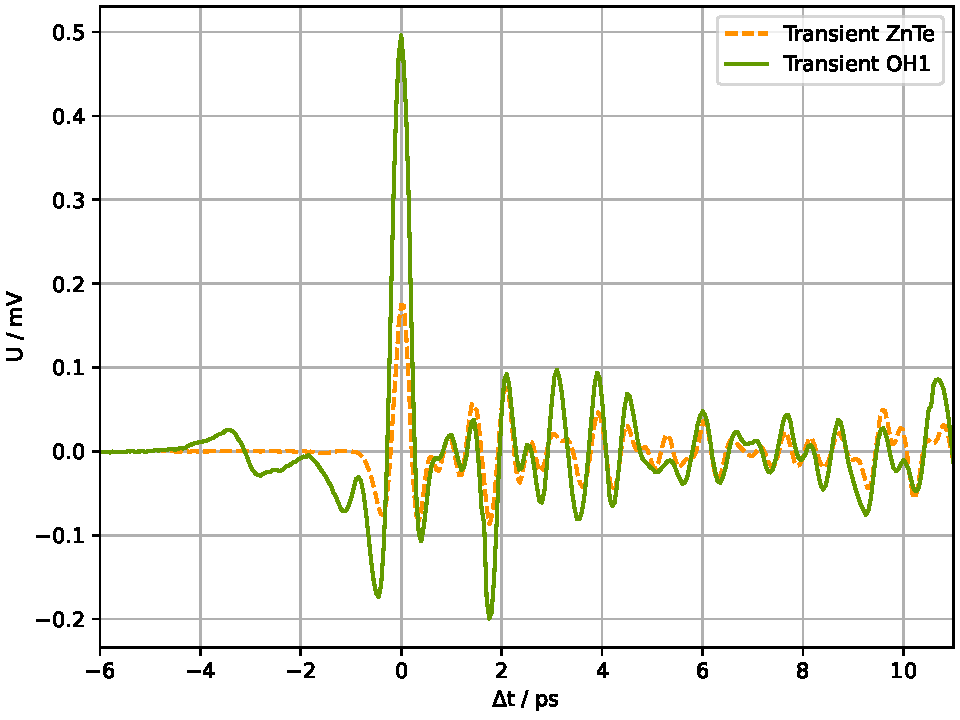
\includegraphics[width=0.8\textwidth]{content/plots/pdf/OH1/470mW,naha,am,fokuspunkt,lange,Messung.pdf}
    \caption{Transient des THz-Pulses bei einer Pump-Leistung von $\SI{470}{\milli\watt}$.
    Die errechneten effektive Leistung, welche den Kristall trifft, beträgt $\SI{86.01}{\milli\watt}$.} % geändert: vorher $\SI{52.64}{\milli\watt}$, neu berechnet mit dem aktualisierten Flächenverhältnis (18,3% statt 11,2%, siehe Kommentar bei "Verhältnis von Strahl zu Kristall" weiter unten) bei $\SI{470}{\milli\watt}$ Pumpleistung: 470*0.183=86.01mW
    \label{fig:OH1T}
\end{figure}

Da der Kristall selbst bei der höchsten Pump-Leistung von $\SI{470}{\milli\watt}$ nicht zerstört wurde, 
wird der Kristall näher an den Fokuspunkt gebracht, um die Leistung pro Fläche zu erhöhen. 
Dabei befand sich der Kristall zu Beginn in einer Entfernung von $\SI{4.5}{\centi\meter}$ zur Linse vor dem Kristall, 
welche eine Brennweite von $\SI{10}{\centi\meter}$ besitzt. 
Nun wird der Kristall auf eine Distanz von $\SI{7}{\centi\meter}$ gebracht. 
Unter der Annahme, dass der Strahl am Fokuspunkt punktförmig ist, ergibt sich an der neuen Position eine Strahlgröße von $\SI{12.246+-0.790}{\milli\meter\squared}$. % geändert: vorher $\SI{20+-4.7}{\milli\meter\squared}$, neu berechnet aus der aktualisierten Strahlfläche in \autoref{sec:spot} (41.159mm^2) über dieselbe Skalierung wie zuvor: alte_Fläche * ((10-7)/(10-4.5))^2 = 41.159*0.2975 = 12.246mm^2, Fehler mit demselben relativen Fehler wie die Fläche in \autoref{sec:spot}
Hierbei ist der vom Kristall ausgefüllte Anteil des Strahls ist von $5,44\,\%$ auf $18,3\,\%$ angewachsen. % geändert: vorher 3,33% auf 11,2%; 5,44%=2.241/41.159, 18,3%=2.241/12.246
Mit dieser Leistung wird ein Transienten-Intervall von $\SIrange{-6}{11}{\pico\second}$ gemessen, 
dieser ist in \autoref{fig:OH1T} zu sehen.


In \autoref{fig:OH1T} ist die Zeit-Null sehr gut zu sehen, mit kleinen Vorschwingungen, die 
möglicherweise auf die nicht phasenangepasste Positionierung des Kristalls zurückzuführen ist. 
Es entstehen nach der Zeit-Null auch Nachschwingungen, die 
auf die natürliche Breite des Pulses und auf die Absorption und Emission durch Wasserdampf in der Luft zurückzuführen ist. 
Dazu ist im Hintergrund der Transient von ZnTe zu sehen, dieser ist signifikant schwächer. 
Sehr interessant ist aber, dass die Nachschwingungen sehr ähnlich, mit geringerer Intensität, verlaufen. 
Das lässt darauf schließen, dass die Nachschwingungen keine Rückreflexionen sind, sondern durch den Wasserdampf entstehen. 


% Referenzkreis: Mitte=(76,72) Radius=61px
% Loch-Fläche: 11681 px
% Kristall-Fläche: 5336 px
% Flächenanteil Kristall/Loch: 45.7 %
% Skalierung: 0.0205 mm/px
% Kristallfläche absolut: 2.241 mm^2
% Kontrollbild gespeichert: mask_vis.jpg

\begin{figure}[p]
    \centering
    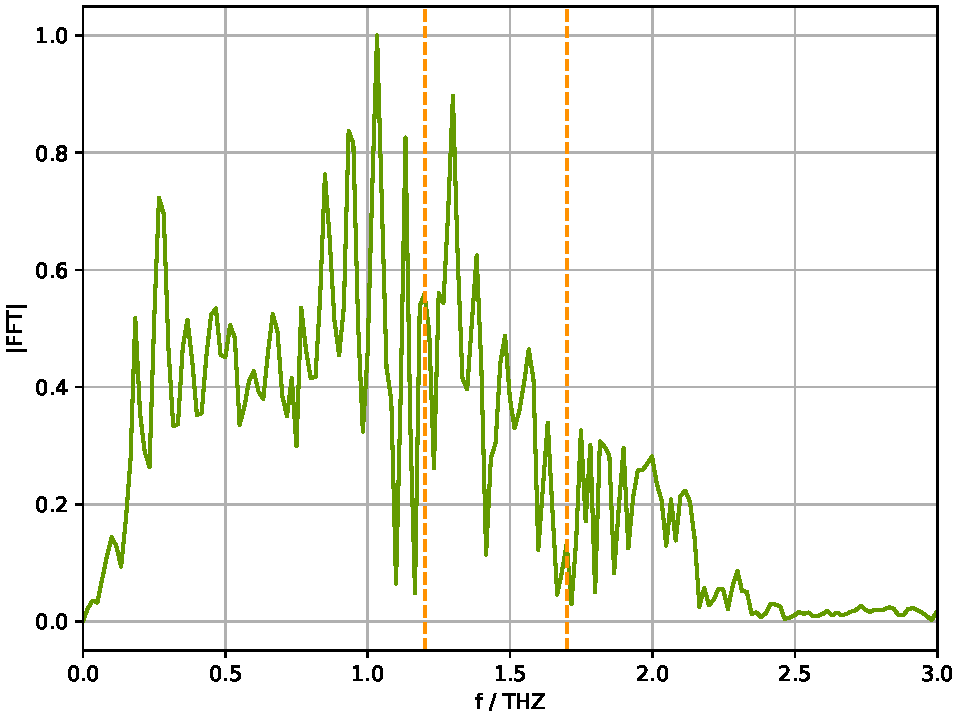
\includegraphics[width=0.8\textwidth]{content/plots/pdf/OH1/470mW,naha,am,fokuspunkt,lange,Messung_fft.pdf}
    \caption{Fouriertransformierte des THz-Pulses bei einer Pump-Leistung von $\SI{470}{\milli\watt}$. 
    Mit der errechneten effektiven Leistung, welche den Kristall trifft, von $\SI{86}{\milli\watt}$.} % geändert: vorher $\SI{52.64}{\milli\watt}$, siehe Kommentar bei \autoref{fig:OH1T}
    \label{fig:OH1f}
\end{figure}

Des Weiteren ist in \autoref{fig:OH1f} die Fouriertransformierte des Transienten zu sehen. 
In dieser lässt sich erkennen, dass in dem THz-Puls Frequenzen von $\SIrange{0.2}{2.2}{THz}$ vorhanden sind, 
was eine Bandbreite von $\SI{2}{THz}$ ergibt. 
Zu beachten ist, dass die Detektion über einen ZnTe-Kristall erfolgt. 
Die gemessene Bandbreite ist somit durch die Detektionsbandbreite des ZnTe begrenzt.
Anschließend wird die maximale Amplitude für die verschiedenen Pump-Leistungen bestimmt. Diese sind 
in \autoref{fig:ampc} aufgetragen. 

% \begin{table}
%     \centering
%     \caption{Peak-to-Peak-Amplitude und daraus bestimmtes Signal-Rausch-Verhältnis der OH1-Transienten bei verschiedenen Pumpleistungen(Auswahl), bezogen auf die einheitliche Rauschreferenz $U_\text{Rausch}=\SI{0.158}{\micro\volt}$ bei $\tau=\SI{450}{ms}$.}
%     \label{tab:SNOH1}
%     \begin{tabular}{S[table-format=3.1] S[table-format=3.1] S[table-format=4.1]}
%         \toprule
%         {$P \mathrel{/} \si{\milli\watt}$} & {$U_\text{ptp} \mathrel{/} \si{\micro\volt}$} & {SNR} \\
%         \midrule
%         8                        & 15.4  & 97.3   \\
%         17,3                     & 7.2   & 45.5   \\
%         24,2                     & 11.2  & 70.9   \\
%         30                       & 77.5  & 490.7  \\
%         38                       & 20.2  & 127.9  \\
%         74                       & 56.4  & 357.2  \\
%         270                      & 88.5  & 559.8  \\
%         350                      & 108.8 & 688.8  \\
%         470                      & 139.2 & 880.8  \\
%         \bottomrule
%     \end{tabular}
% \end{table}



Hierbei wird für den OH1-Kristall nicht die Pumpleistung genutzt, sondern die Leistung pro Fläche multipliziert mit der Fläche des 
Kristalls. 
Die Leistungsdichte wurde in \autoref{sec:spot} zu $\SI{0.838+-0.054}{\milli\watt\per\milli\meter\squared}$ bestimmt und die Fläche des
Kristalls mittels Mikroskopaufnahmen zu $\SI{2.241}{\milli\meter\squared}$ bestimmt. 


\begin{figure}
    \centering
    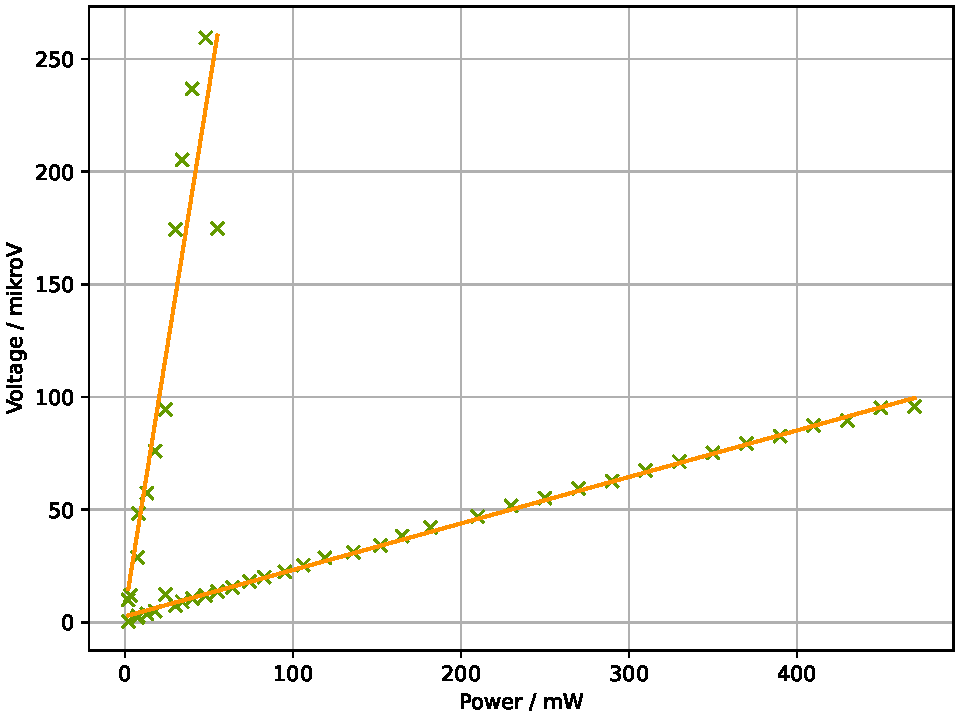
\includegraphics[width=0.8\textwidth]{content/plots/pdf/amplitude_comb.pdf}
    \caption{Vergleich der maximalen Amplitude des THz-Transienten von ZnTe und OH1.
    Als Vergleich wird jeweils eine Ausgleichsgerade durch beide Messreihen gelegt.}
    \label{fig:ampc}
\end{figure}

Da der Kristall eine deutlich geringere Fläche als der ZnTe-Kristall besitzt und somit auch weniger Leistung aufnimmt, zeigt sich 
dies in \autoref{fig:ampc}.
Das ist erkennbar dadurch, dass die maximalen Amplituden des OH1-Kristalls im Gegensatz zu ZnTe alle bei geringen Leistungen liegen. 
Des Weiteren ist die Amplitude der von OH1 erzeugten THz-Strahlung weniger steil, als die des ZnTe ansteigt. 
Hierbei kann der in \autoref{sec:ME} bestimmte nichtlineare Koeffizient hinzugezogen werden. 
Denn die bestimmten maximalen Amplituden sind linear abhängig von diesem Koeffizienten. 
Als Verhältnis zeigt sich $\frac{d_\text{THz}^\text{OH1}}{d_\text{THz}^\text{ZnTe}} \approx \SI{4.2}{}$, somit sollte nach 
den theoretischen Werten die Steigung der Geraden bei den OH1‑Messwerten um den Faktor $4,2$ größer sein als die der Geraden des ZnTe. 
Aus \autoref{fig:ampc} ergeben sich $m_\text{ZnTe}= \SI{4.6}{\micro\volt\per\milli\watt}$ und $m_\text{OH1}= \SI{3.8}{\micro\volt\per\milli\watt}$. % geändert: vorher m_OH1=3.1. m_ZnTe bleibt gleich (ZnTe-Fit hängt nicht von der Intensitaet ab). m_OH1 analytisch abgeleitet, NICHT durch Neu-Ausführen von amplitude_combined.py bestimmt: die x-Werte des OH1-Fits skalieren linear mit der Intensitaetskonstante (siehe Kommentar dort), Skalierungsfaktor k=0.0838/0.103=0.8139, neue Steigung = alte Steigung/k = 3.1/0.8139=3.809≈3.8. Bitte mit echtem Skriptlauf (make) verifizieren.
Hierbei ist der Faktor $0,83$, somit deutlich kleiner als erwartet. % geändert: vorher 0,67 (=3.1/4.6); neu 0,83 (=3.8/4.6) -- Kernaussage (deutlich kleiner als der erwartete Faktor 4,2) bleibt unverändert gültig
Eine Erklärung dafür ist, dass OH1 explizit für die THz‑Generation mit einer Pump-Wellenlänge von $\lambda \approx \SI{1300}{\nano\meter}$ optimiert wurde 
und somit auch die gemessenen Werte für den nichtlinearen Koeffizienten für diesen Bereich gelten. 
Durch nicht vorhandene Phasenanpassung bei der genutzten Pump-Wellenlänge kann sich die Intensität der erzeugten THz-Strahlung verringern.
Als größeren limitierenden Faktor spielt die Detektionsbandbreite des Detektionskristalls. 
Denn der ZnTe-Kristall kann keine Frequenzen oberhalb von $\SI{2.5}{THz}$ detektieren. 
Da OH1 aber theoretisch deutlich breitbandigere und höhere Frequenzen generiert, wird diese Leistung nicht messbar.
Dazu sind in den geplotteten Werten des ZnTe-Kristalls die in \autoref{sec:AZnTe} erwähnten abweichenden Messwerte zwischen $\SIrange{30}{48}{\milli\watt}$ erkennbar.

\section{THz-Generation mit BNA}
\label{sec:ABNA}

Für BNA wurde wie bei den anderen Materialien zuvor ein großer Bereich der Verzögerungsstrecke abgesucht und anschließend immer die Pump-Leistung von $\SIrange{2.2}{480}{\milli\watt}$ erhöht. 
\autoref{fig:BNAt} zeigt den Transienten bei der höchsten Pump-Leistung. Dabei ist kein Signal oberhalb des Rauschniveaus erkennbar.
Dies deutet zunächst darauf hin, dass mit der genutzten Probe keine signifikante 
THz-Strahlung erzeugt werden konnte. 
Die Gründe hierfür werden im Folgenden erläutert.

\begin{figure}
    \centering
    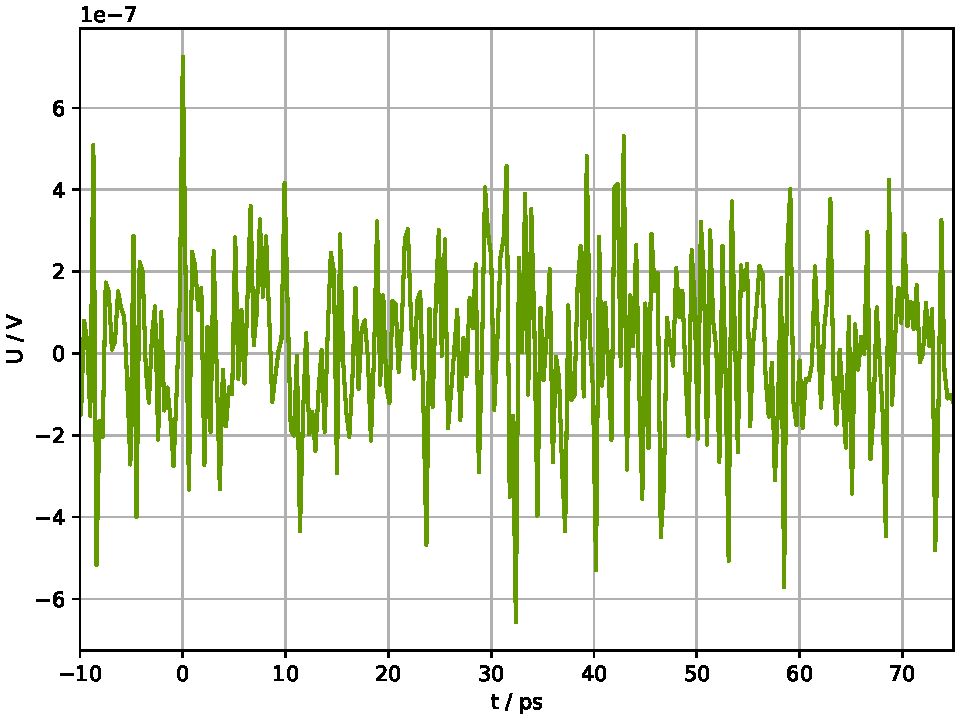
\includegraphics[width=0.8\textwidth]{content/plots/pdf/BNA/480mW,real.pdf}
    \caption{Gemessener Transient bei einer Pumpleistung von $\SI{480}{\milli\watt}$.
    Dabei ist kein Signal oberhalb des Rauschniveaus zu erkennen.}
    \label{fig:BNAt}
\end{figure}

Die Proben sind sehr kleine, pulverartige Kristalle, wobei bei einzelnen Kristalliten nicht sicher feststellbar war, 
ob es sich tatsächlich um Einzelkristalle handelt; ihr Durchmesser betrug maximal $\SI{2}{\milli\meter}$.
Die genutzte Probe wurde in einem Mikroskop auf Unebenheiten und andere Anomalien untersucht. 
In \autoref{fig:my8} ist eine achtfache Vergrößerung der Probe zu sehen. 
In dieser sind Unebenheiten und verschiedene Schichten zu sehen. 
Eingezeichnet ist eine dieser Unebenheiten, wobei diese eine Länge von $\SI{0.228}{\milli\meter}$ besitzt. 
Das hat zur Folge, dass, wenn viele verschiedene Kristalle in der Probe vorhanden sind, diese auch immer unterschiedliche Ausrichtungen haben. 
Durch diese Ausrichtung erzeugen die einzelnen Kristalle für sich THz-Strahlung, 
aber diese haben jeweils eine unterschiedliche Polarisationsrichtung und Phase relativ zueinander. 
Die beobachteten Schichten und Unebenheiten deuten darauf hin, dass die Probe aus vielen Kristalliten mit zufälligen Orientierungen besteht.
Dadurch mittelt sich die Überlagerung der von den einzelnen Kristalliten erzeugten THz-Felder näherungsweise zu null.
Die optisch aktive Fläche des Kristalls beträgt $\SI{6.28}{\milli\meter\squared}$.
Somit ist die effektive Leistung, 
welche auf den Kristall trifft, um einen Faktor 3 größer als die bei OH1, aber immer noch um den Faktor 6,5 kleiner als bei ZnTe.
Somit kann durch die Qualität der Probe keine Aussage über die Nutzbarkeit des Materials zur Erzeugung von THz-Strahlung in 
dem verwendeten Aufbau getätigt werden. 



%5,632/2560=0,0022mm/pixel
%8x vergrößerung also 0,000275 mm/pixel
%574*599=829,62Pixel
%Länge = 0,228mm


\begin{figure}
    \centering
    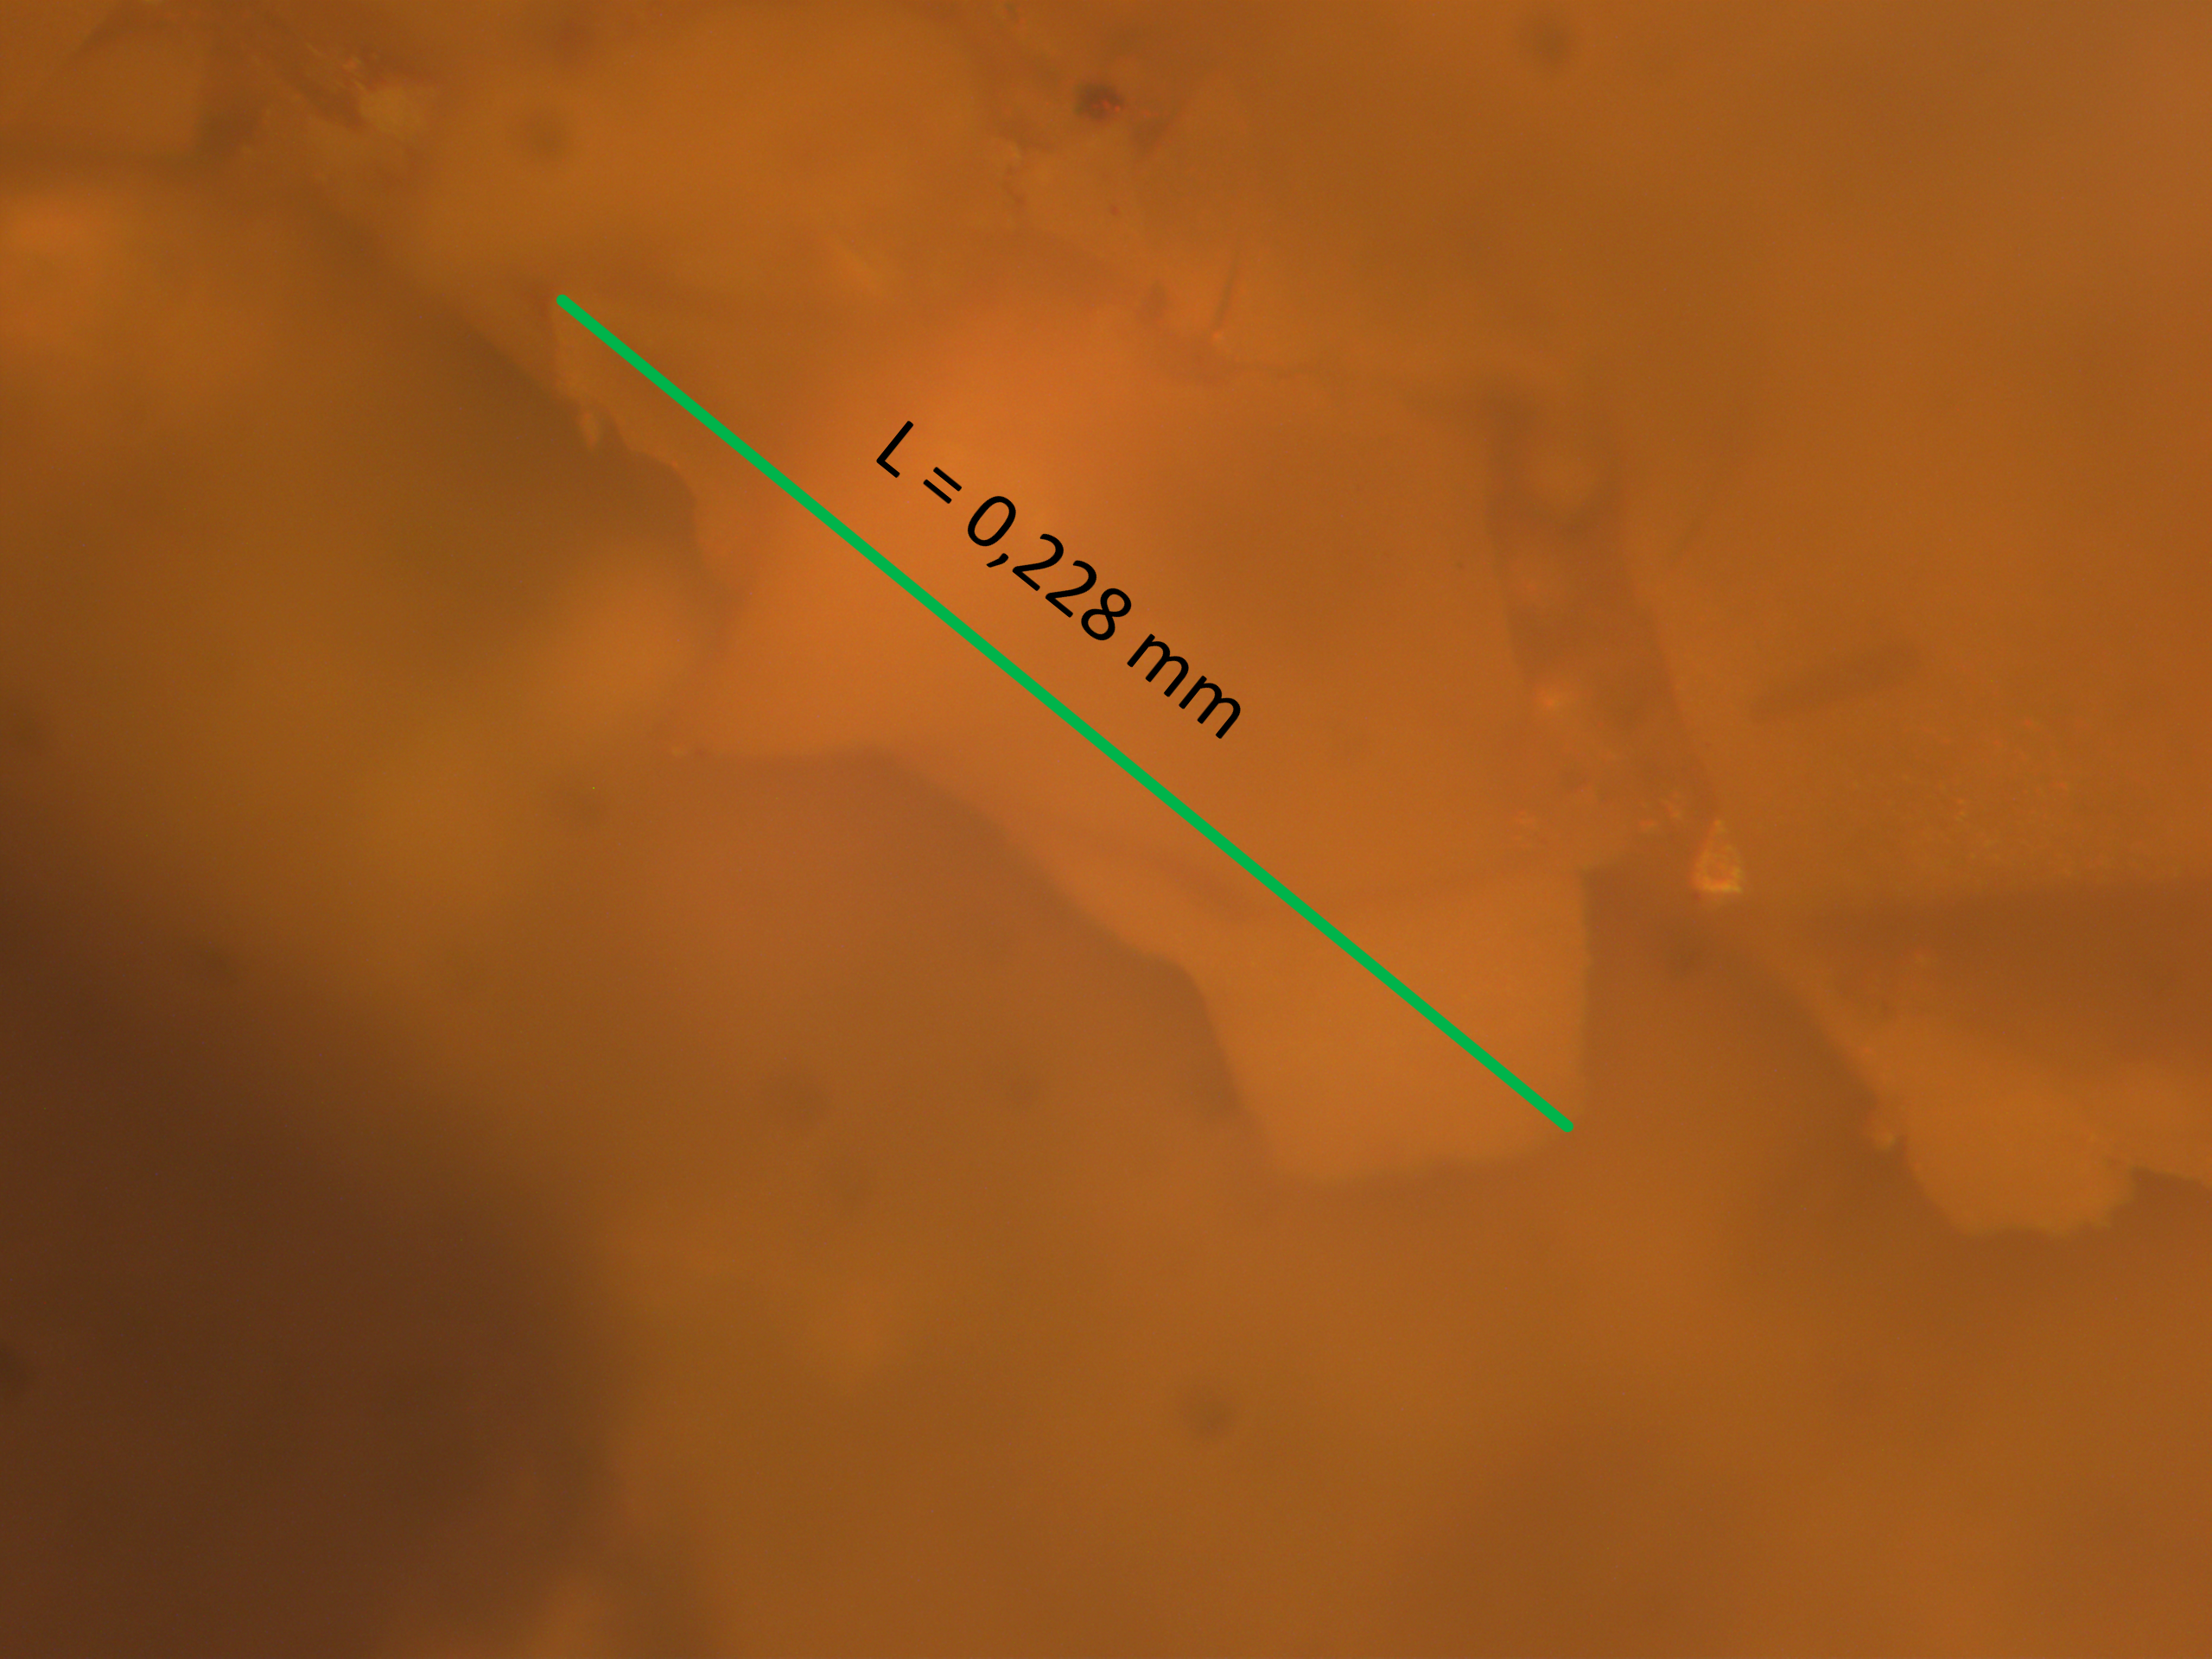
\includegraphics[width=0.8\textwidth]{content/bilder/mikroskop/yellow_drauflicht_8x.png}
    \caption{Achtfache Vergrößerung der Genutzten BNA Probe, mit eingezeichneter Unebenheit mit einer Länge $L=\SI{0.228}{mm}$.}
    \label{fig:my8}
\end{figure}


% \begin{figure}
%     \centering
%     \includegraphics[width=0.8\textwidth]{content/plots/build/OH1/transients/202608071724_1Dx1D_756ed8_470mW_naha_am_fokuspunkt_lange_Messung.pdf}
%     \caption{Vergleich der Rauschspannung mit und ohne eingeschaltetem Laser.}
%     \label{fig:tcc}
% \end{figure}
% \begin{figure}
%     \centering
%     \includegraphics[width=0.8\textwidth]{content/plots/build/OH1/transients/202608071709_1Dx1D_40e4a3_470mW_naeher_am_Fokus2.pdf}
%     \caption{Vergleich der Rauschspannung mit und ohne eingeschaltetem Laser.}
%     \label{fig:tcc}
% \end{figure}

% \begin{figure}
%     \centering
%     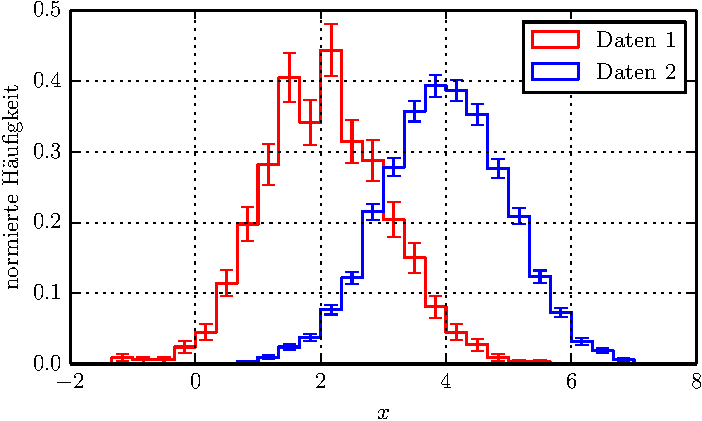
\includegraphics[\textwidth]{./Plots/Histogramm.pdf}
%     \caption{Ein Histogramm mit Fehlerbalken für zwei Datensätze, Schriftgröße und -art entsprechen der des Dokuments.}
%     \label{fig:bsp}
% \end{figure}


